\documentclass[10pt]{article}\usepackage[]{graphicx}\usepackage[]{color}
%% maxwidth is the original width if it is less than linewidth
%% otherwise use linewidth (to make sure the graphics do not exceed the margin)
\makeatletter
\def\maxwidth{ %
  \ifdim\Gin@nat@width>\linewidth
    \linewidth
  \else
    \Gin@nat@width
  \fi
}
\makeatother

\definecolor{fgcolor}{rgb}{0.345, 0.345, 0.345}
\newcommand{\hlnum}[1]{\textcolor[rgb]{0.686,0.059,0.569}{#1}}%
\newcommand{\hlstr}[1]{\textcolor[rgb]{0.192,0.494,0.8}{#1}}%
\newcommand{\hlcom}[1]{\textcolor[rgb]{0.678,0.584,0.686}{\textit{#1}}}%
\newcommand{\hlopt}[1]{\textcolor[rgb]{0,0,0}{#1}}%
\newcommand{\hlstd}[1]{\textcolor[rgb]{0.345,0.345,0.345}{#1}}%
\newcommand{\hlkwa}[1]{\textcolor[rgb]{0.161,0.373,0.58}{\textbf{#1}}}%
\newcommand{\hlkwb}[1]{\textcolor[rgb]{0.69,0.353,0.396}{#1}}%
\newcommand{\hlkwc}[1]{\textcolor[rgb]{0.333,0.667,0.333}{#1}}%
\newcommand{\hlkwd}[1]{\textcolor[rgb]{0.737,0.353,0.396}{\textbf{#1}}}%
\let\hlipl\hlkwb

\usepackage{framed}
\makeatletter
\newenvironment{kframe}{%
 \def\at@end@of@kframe{}%
 \ifinner\ifhmode%
  \def\at@end@of@kframe{\end{minipage}}%
  \begin{minipage}{\columnwidth}%
 \fi\fi%
 \def\FrameCommand##1{\hskip\@totalleftmargin \hskip-\fboxsep
 \colorbox{shadecolor}{##1}\hskip-\fboxsep
     % There is no \\@totalrightmargin, so:
     \hskip-\linewidth \hskip-\@totalleftmargin \hskip\columnwidth}%
 \MakeFramed {\advance\hsize-\width
   \@totalleftmargin\z@ \linewidth\hsize
   \@setminipage}}%
 {\par\unskip\endMakeFramed%
 \at@end@of@kframe}
\makeatother

\definecolor{shadecolor}{rgb}{.97, .97, .97}
\definecolor{messagecolor}{rgb}{0, 0, 0}
\definecolor{warningcolor}{rgb}{1, 0, 1}
\definecolor{errorcolor}{rgb}{1, 0, 0}
\newenvironment{knitrout}{}{} % an empty environment to be redefined in TeX

\usepackage{alltt}

\usepackage{amsmath,amssymb,amsthm}
\usepackage{fancyhdr,url,hyperref}
\usepackage{graphicx,xspace}
\usepackage{tikz}
\usetikzlibrary{shapes,arrows,decorations.pathmorphing,backgrounds,positioning,fit,through}

\oddsidemargin 0in  %0.5in
\topmargin     0in
\leftmargin    0in
\rightmargin   0in
\textheight    9in
\textwidth     6in %6in
%\headheight    0in
%\headsep       0in
%\footskip      0.5in

\newtheorem{thm}{Theorem}
\newtheorem{cor}[thm]{Corollary}
\newtheorem{obs}{Observation}
\newtheorem{lemma}{Lemma}
\newtheorem{claim}{Claim}
\newtheorem{definition}{Definition}
\newtheorem{question}{Question}
\newtheorem{answer}{Answer}
\newtheorem{problem}{Problem}
\newtheorem{solution}{Solution}
\newtheorem{conjecture}{Conjecture}

\pagestyle{fancy}

\lhead{\textsc{Prof. McNamara}}
\chead{\textsc{SDS/MTH 291: Lecture notes}}
\lfoot{}
\cfoot{}
%\cfoot{\thepage}
\rfoot{}
\renewcommand{\headrulewidth}{0.2pt}
\renewcommand{\footrulewidth}{0.0pt}

\newcommand{\ans}{\vspace{0.25in}}
\newcommand{\R}{{\sf R}\xspace}
\newcommand{\cmd}[1]{\texttt{#1}}
\DeclareMathOperator{\Ex}{\mathbb{E}}
\DeclareMathOperator{\Var}{\text{Var}}
\DeclareMathOperator{\X}{\mathbf{X}}
\DeclareMathOperator{\Hatmat}{\mathbf{H}}

\rhead{\textsc{November 29, 2016}}
\IfFileExists{upquote.sty}{\usepackage{upquote}}{}
\begin{document}

\paragraph{Agenda}
\begin{enumerate}
  \itemsep0em
  \item Logistic Regression
  \item Assessing Fit in Logistic Regression
\end{enumerate}



\paragraph{Binary response}
	\begin{itemize}
		\item What do to when response variable $p$ is \emph{binary}?
		\item Linear model will produce illogical estimates (eg. $\hat{p} > 1$ or $ \hat{p} < 0$)
		\end{itemize}
		
\begin{knitrout}\footnotesize
\definecolor{shadecolor}{rgb}{0.969, 0.969, 0.969}\color{fgcolor}\begin{kframe}
\begin{alltt}
\hlkwd{require}\hlstd{(mosaic)}
\hlkwd{require}\hlstd{(Stat2Data)}
\hlkwd{data}\hlstd{(Whickham)}
\hlstd{Whickham} \hlkwb{=} \hlstd{Whickham} \hlopt
  \hlkwd{mutate}\hlstd{(}\hlkwc{isAlive} \hlstd{=} \hlnum{2} \hlopt{-} \hlkwd{as.numeric}\hlstd{(outcome))}
\hlkwd{xyplot}\hlstd{(isAlive}\hlopt{~}\hlkwd{jitter}\hlstd{(age),} \hlkwc{data}\hlstd{=Whickham,} \hlkwc{pch}\hlstd{=}\hlnum{19}\hlstd{,} \hlkwc{cex}\hlstd{=}\hlnum{1.5}\hlstd{,} \hlkwc{alpha}\hlstd{=}\hlnum{0.05}\hlstd{,} \hlkwc{col}\hlstd{=}\hlstr{"black"}\hlstd{)}
\end{alltt}
\end{kframe}
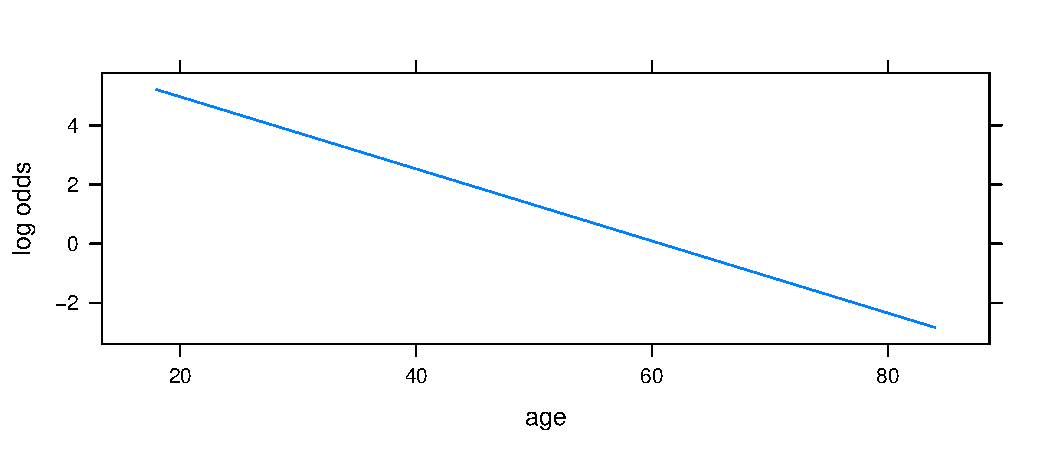
\includegraphics[width=\maxwidth]{figure/unnamed-chunk-2-1} 

\end{knitrout}

\begin{knitrout}\footnotesize
\definecolor{shadecolor}{rgb}{0.969, 0.969, 0.969}\color{fgcolor}\begin{kframe}
\begin{alltt}
\hlkwd{plotModel}\hlstd{(}\hlkwd{lm}\hlstd{(isAlive}\hlopt{~}\hlstd{age,} \hlkwc{data}\hlstd{=Whickham),} \hlkwc{pch}\hlstd{=}\hlnum{19}\hlstd{)}
\end{alltt}
\end{kframe}
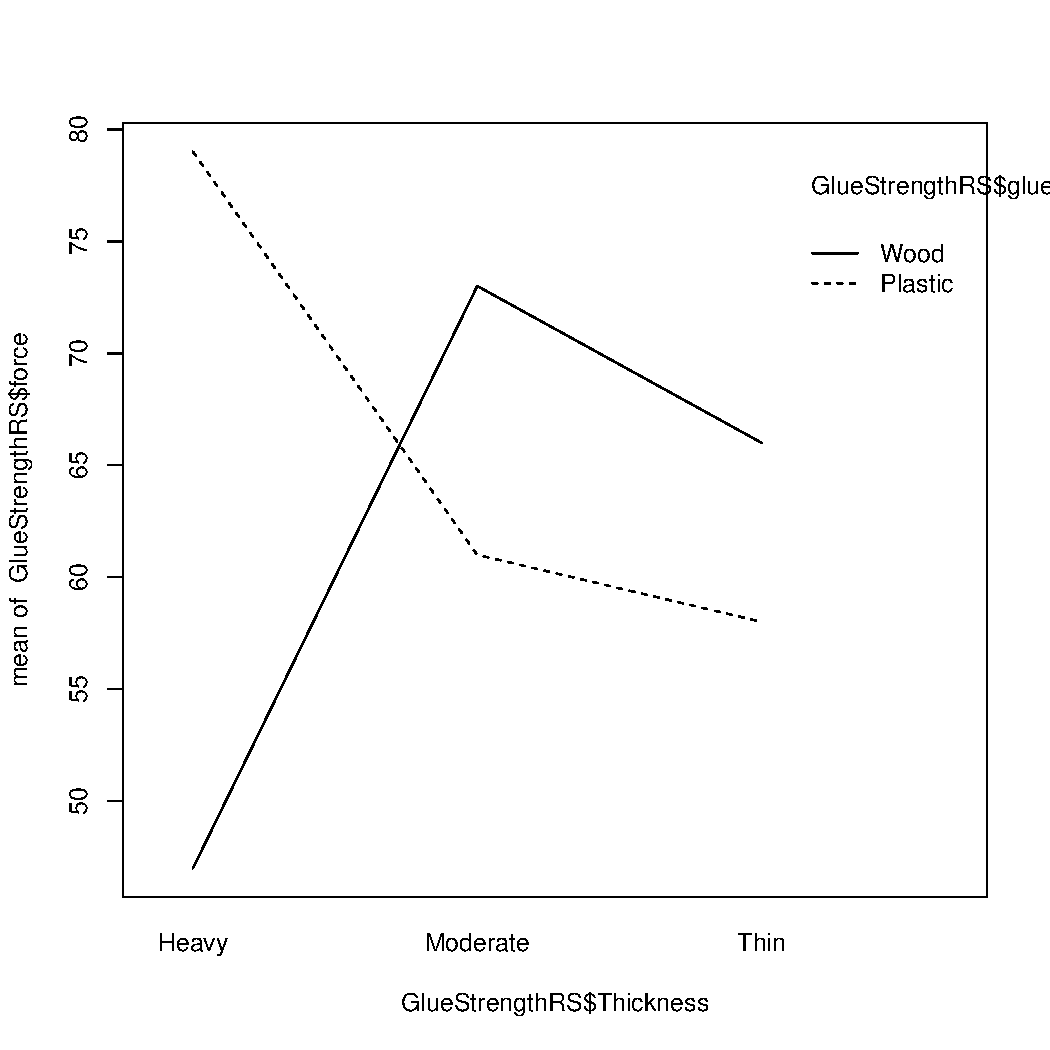
\includegraphics[width=\maxwidth]{figure/unnamed-chunk-3-1} 

\end{knitrout}

This doesn't make sense outside the $[0,1]$ range. One solution might be to summarize the data to be frequencies at each age. 
\begin{knitrout}\footnotesize
\definecolor{shadecolor}{rgb}{0.969, 0.969, 0.969}\color{fgcolor}\begin{kframe}
\begin{alltt}
\hlstd{alive} \hlkwb{=} \hlstd{Whickham} \hlopt
  \hlkwd{group_by}\hlstd{(age, isAlive)} \hlopt
  \hlkwd{summarize}\hlstd{(}\hlkwc{total} \hlstd{=} \hlkwd{n}\hlstd{())} \hlopt
  \hlkwd{mutate}\hlstd{(}\hlkwc{freq} \hlstd{= total} \hlopt{/} \hlkwd{sum}\hlstd{(total))} \hlopt
  \hlkwd{filter}\hlstd{(isAlive}\hlopt{==}\hlnum{1}\hlstd{)}
\hlkwd{xyplot}\hlstd{(freq}\hlopt{~}\hlstd{age,} \hlkwc{data}\hlstd{=alive,}\hlkwc{pch}\hlstd{=}\hlnum{19}\hlstd{,} \hlkwc{col}\hlstd{=}\hlstr{"black"}\hlstd{)}
\end{alltt}
\end{kframe}
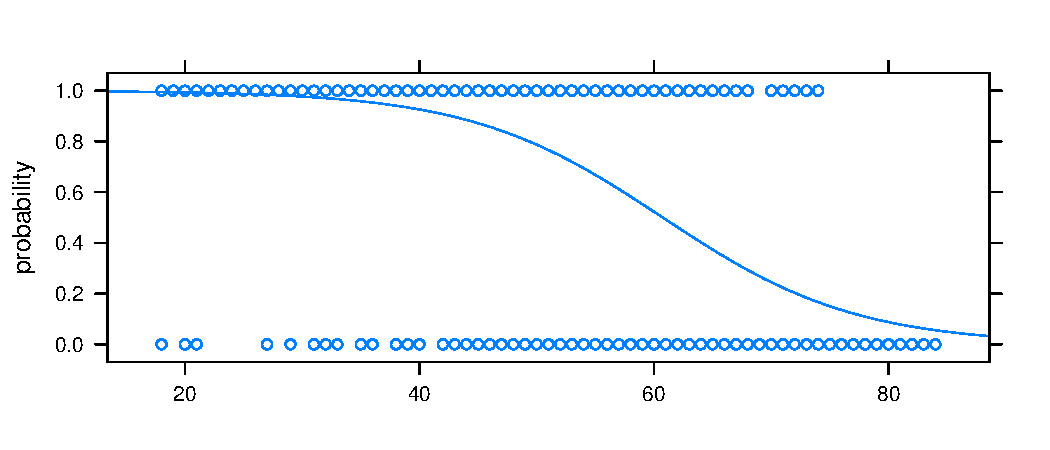
\includegraphics[width=\maxwidth]{figure/unnamed-chunk-4-1} 

\end{knitrout}

\begin{knitrout}\footnotesize
\definecolor{shadecolor}{rgb}{0.969, 0.969, 0.969}\color{fgcolor}\begin{kframe}
\begin{alltt}
\hlkwd{xyplot}\hlstd{(freq}\hlopt{~}\hlstd{age,} \hlkwc{data}\hlstd{=alive,} \hlkwc{pch}\hlstd{=}\hlnum{19}\hlstd{,} \hlkwc{type}\hlstd{=}\hlkwd{c}\hlstd{(}\hlstr{"p"}\hlstd{,} \hlstr{"r"}\hlstd{))}
\end{alltt}
\end{kframe}
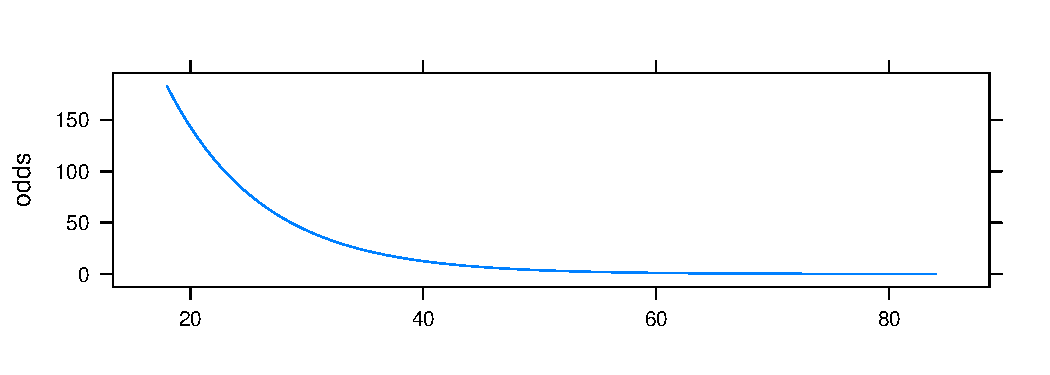
\includegraphics[width=\maxwidth]{figure/unnamed-chunk-5-1} 

\end{knitrout}

But, this still has strange interpretations. 

\paragraph{Logistic Regression}
What's the solution? Logistic regression! This uses the logit function as a `link.'
	\begin{itemize}
		\item logit produces S-curve that is always in $[0,1]$
		\item Fit via \emph{maximum likelihood estimation}, not OLS
		\item No such thing as $R^2$ or sum of squares
	\end{itemize}

\clearpage
	\paragraph{Warmup-- probability and odds}
Probabilities and odds express the same information, but have different interpretation. Lets fill in this chart to help warm up our intuition about their relationship.
\begin{center}
\begin{tabular}{|c|c|}
\hline
Probability of success ($\pi$) & Odds ($\pi/(1-\pi)$) \\
\hline
1/2 & 1/1 \\
& \\
\hline
1/3 & 1/2 \\
& \\
\hline
1/4 & \\
& \\
\hline 
1/5 & \\
& \\
\hline 
2/3 & \\
& \\
\hline 
3/4 & \\
& \\
\hline
\end{tabular}
\end{center}

\paragraph{``Spaces''}

We often talk about three `spaces' for logistic regression. These are just different ways of writing the same thing, but they have different interpretations so they are useful for different tasks. 

\begin{itemize}
\item Log odds space
	\begin{eqnarray*}
			\log \left( \frac{\pi}{1-\pi} \right) &=& \beta_0 + \beta_1\cdot X \\
		\end{eqnarray*}
		
		Thinking about log odds is useful when you want a linear form of a regression line. You can interpret the coefficients in the standard way we have been doing for linear regression, ``A one unit increase in $x$ is associated with a $\beta_1$ increase in the log odds of $y$''
		
\begin{knitrout}\footnotesize
\definecolor{shadecolor}{rgb}{0.969, 0.969, 0.969}\color{fgcolor}\begin{kframe}
\begin{alltt}
\hlstd{m1} \hlkwb{=} \hlkwd{glm}\hlstd{(isAlive}\hlopt{~}\hlstd{age,} \hlkwc{data}\hlstd{=Whickham,} \hlkwc{family}\hlstd{=binomial)}
\hlkwd{xyplot}\hlstd{(}\hlkwd{log}\hlstd{(}\hlkwd{fitted.values}\hlstd{(m1)}\hlopt{/}\hlstd{(}\hlnum{1}\hlopt{-}\hlkwd{fitted.values}\hlstd{(m1)))}\hlopt{~}\hlstd{age,} \hlkwc{data}\hlstd{=Whickham,} \hlkwc{type}\hlstd{=}\hlkwd{c}\hlstd{(}\hlstr{"l"}\hlstd{),}\hlkwc{ylab}\hlstd{=}\hlstr{"log odds"}\hlstd{)}
\end{alltt}
\end{kframe}
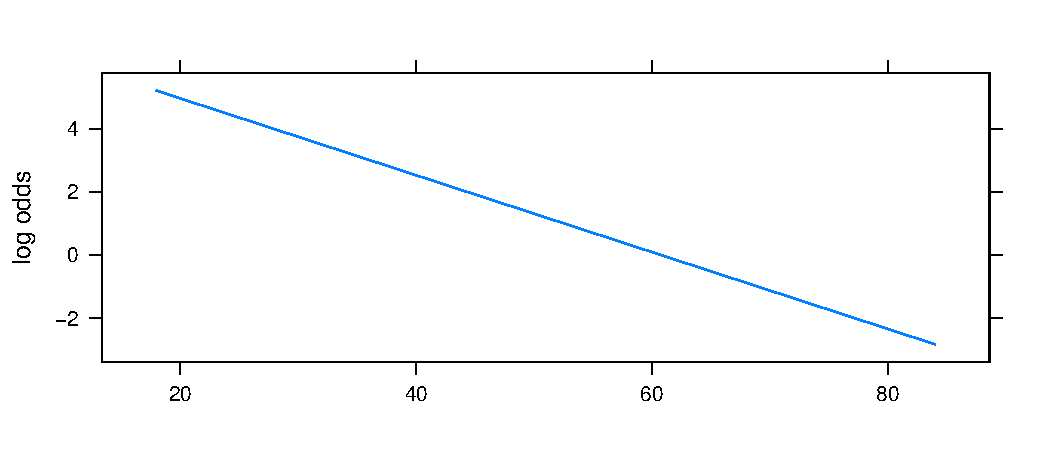
\includegraphics[width=\maxwidth]{figure/unnamed-chunk-6-1} 

\end{knitrout}
\clearpage
		\item Odds space
		
		\begin{eqnarray*}
	    \frac{\pi}{1-\pi} &=& e^{\beta_0 + \beta_1\cdot X}
		\end{eqnarray*}

Odds are useful when you want to interpret the slope coefficient. We can use the interpretation, ``A one unit increase in $x$ is associated with changing $y$ by a factor of $e^{\beta_1}$. 

\begin{knitrout}\footnotesize
\definecolor{shadecolor}{rgb}{0.969, 0.969, 0.969}\color{fgcolor}\begin{kframe}
\begin{alltt}
\hlkwd{xyplot}\hlstd{(}\hlkwd{fitted.values}\hlstd{(m1)}\hlopt{/}\hlstd{(}\hlnum{1}\hlopt{-}\hlkwd{fitted.values}\hlstd{(m1))}\hlopt{~}\hlstd{age,} \hlkwc{data}\hlstd{=Whickham,}  \hlkwc{type}\hlstd{=}\hlstr{"spline"}\hlstd{,} \hlkwc{ylab}\hlstd{=}\hlstr{"odds"}\hlstd{)}
\end{alltt}
\end{kframe}
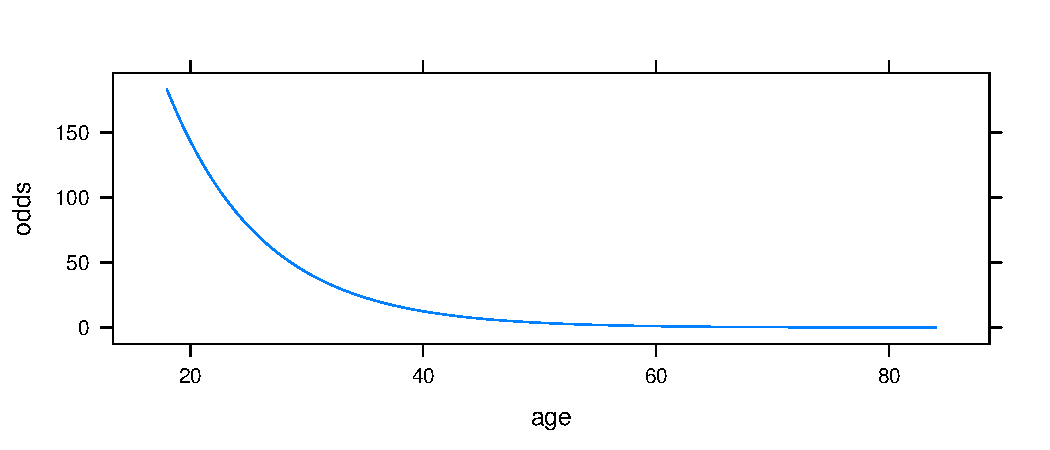
\includegraphics[width=\maxwidth]{figure/unnamed-chunk-7-1} 

\end{knitrout}

\item Probability space
	\begin{eqnarray*}
			\pi &=& \frac{e^{\beta_0 + \beta_1\cdot X}}{1 + e^{\beta_0 + \beta_1\cdot X}}
		\end{eqnarray*}
		The probability form is how the model gets fit, but it does not have an easy interpretation for what happens with a change in $x$. 
\begin{knitrout}\footnotesize
\definecolor{shadecolor}{rgb}{0.969, 0.969, 0.969}\color{fgcolor}\begin{kframe}
\begin{alltt}
\hlkwd{plotModel}\hlstd{(m1,} \hlkwc{ylab}\hlstd{=}\hlstr{"probability"}\hlstd{)}
\end{alltt}
\end{kframe}
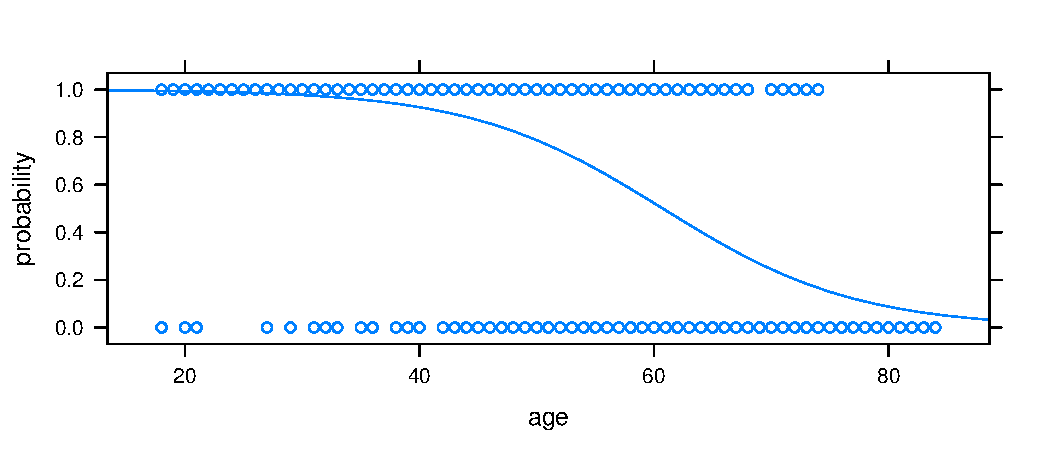
\includegraphics[width=\maxwidth]{figure/unnamed-chunk-8-1} 

\end{knitrout}

\end{itemize}



	
% 	pg. 455, ``linear on the right, log(odds) on the left``
% 	Should do the math to go from log(odds) to probability and vice versa
% 	Do the math to show that the 50\% point is at $x=-\beta_0/\beta_1$
% 	Point out which pieces of this correspond to the CFAU framework. E.g., inference. 
%   pg. 525, comparison of tests and intervals for ordinary regression and logistic regression

\end{document}
